\chapter{Ejecución y Pruebas}


\subsubsection{Instrucciones de uso y ejecución}

En los siguiente apartados mostramos los pasos a seguir para la obtención de resultados en MOSS y en JPLAG.

\section{Ejecución en MOSS}

Siguiendo las instrucciones en \cite{Moss_web} y en \cite{instrucciones_moss} sabemos que, para poder comunicarnos en el servidor de MOSS y mandarle los archivos, necesitaremos un script en Perl.
\newline
Para obtener este script enviamos un mensaje por correo electrónico a 
\newline 
moss@moss.stanford.edu con lo siguiente en el cuerpo del mensaje:

\begin{center}
registeruser
\\mail usuario@dominio
\end{center}

En nuestro caso pondremos antoniojrp@correo.ugr.es en la parte de usuario@dominio.
\newline
Unos cinco minutos después del envío de este mensaje recibiremos una respuesta automática del servidor en nuestro correo con el script que necesitamos y con instrucciones de su uso.
En el script se detalla que podemos compartir este script con otros profesores de programación pero que por favor no lo compartamos en un sitio de acceso público (''Feel free to share this script with other instructors of programming classes, but please do not place the script in a publicly accessible place.''), por esta razón no mostramos el contenido completo del script en esta memoria.

\bigskip
Ahora que tenemos el script, lo colocamos en el directorio donde tenemos los archivos o las carpetas de los archivos que queremos comparar, para mayor comodidad a la hora de escribir las rutas de los archivos al llamar al script.
\newline
Nos situamos con la terminal (este script funciona en Unix, en caso estar en Windows se tendrá que usar Cygwin) en el directorio donde está el script y ejecutamos los siguientes comandos:

\bigskip

Para modo Matlab:
\begin{center}
\begin{lstlisting}[language=bash]
$ ./moss -l matlab -c "Entrega X" "Entrega X"/*.r "Entrega X"/*.R
\end{lstlisting}
\end{center}


Para modo texto plano:
\begin{center}
\begin{lstlisting}[language=bash]
$ ./moss -l ascii -c "Entrega X" "Entrega X"/*.r "Entrega X"/*.R
\end{lstlisting}
\end{center}

Entrega X es la entrega de alumnos que queremos evaluar actualmente, ya que en nuestro caso hay un total de 7 entregas diferentes ( siete trabajos diferentes con más de 30 archivos de ejercicios de alumnos en R en cada uno), y hemos nombrado el directorio donde se encuentran cada una de las entregas ''Entrega 1'', ''Entrega 2'', ''Entrega 3'', etc hasta siete entregas.

\bigskip

\subsubsection{Explicación de opciones:}

Con la opción -l especificamos el lenguaje en el que (supuestamente) están los archivos para que MOSS lo tenga en cuenta en su algoritmo. En nuestro caso hemos decidido realizar las pruebas como si los archivos estuvieran escritos en texto plano y en Matlab (dado que es el más similar a R de todas las posibles opciones). Si esta opción se deja vacía, MOSS supondrá que los archivos están en C.

\bigskip

Con la opción -c le asocia un nombre a los resultados que se generan. En nuestro caso le asociamos el número de la entrega.

\bigskip

Entre las opciones que no hemos especificado tenemos:

\begin{itemize}
\item -m: Especifica el número máximo de veces que un mismo fragmento de código tiene que aparecer para que se ignore en los emparejamientos. Por defecto esta opción tiene el valor 10.
\item -d: Especifica que los archivos a evaluar se agrupan por directorio y no por archivos individuales, es decir, cada alumno es un directorio completo lleno de archivos y se compara entre directorios.
\item -b: Nos permite especificar un archivo base. El código que tengan en común el resto de archivos con el archivo base no se tendrá en cuenta en los emparejamientos.
\end{itemize}

Al ejecutar estos comandos, le enviamos los archivos al servidor y obtenemos un enlace como el siguiente:
\begin{center}
http://moss.stanford.edu/results/169343157
\end{center}
Es posible que en el momento que se lea esto el enlace de ejemplo no exista ya que el servidor borra los resultados 15 días después de generarlos.
\newline
En nuestro caso han tardado de media un minuto en generarse, variando en función del tamaño de los archivos de la entrega (treinta segundos para la entrega más corta y un minuto y cuarenta segundos para la más larga). 
\newline
Al acceder a este enlace podemos ver en nuestro navegador una página principal con los resultados, en el caso por ejemplo de la Entrega 2, hemos obtenido la página de resultados de la Figura \ref{fig:entrega2_MOSS_1}.
\newline
La página muestra la fecha en la que fue generada, las opciones de ejecución elegidas a la hora de ejecutar el script y la etiqueta que le asociamos con la opción -c.
\newline
Seguido de esto tenemos seis links de ayuda con las bases de cómo interpretar los resultados, contacto y créditos.
\newline
El resto de la página contiene una tabla de pares de archivos con código similar, ordenado por la cantidad de código en común entre estos.
\newline
Al final del nombre de cada archivo está el porcentaje del código de ese archivo que se considera coincidente con el del otro en su misma línea.
\newline
Por último cabe mencionar que la columna ''Lines Matched'' contiene el número aproximado de lineas de código emparejadas entre los archivos de la fila.


\begin{figure}[] %con el [H] le obligamos a situar aquí la figura
\centering
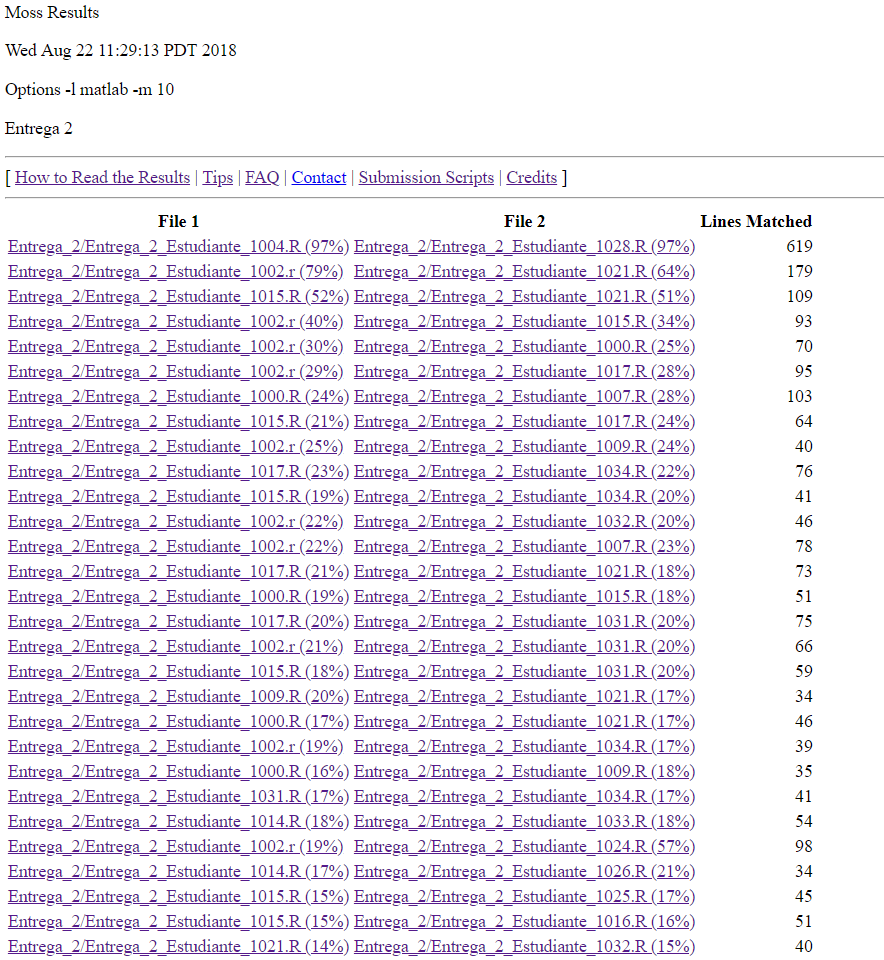
\includegraphics[ width=13cm, height=15cm]{imagenes/entrega2_MOSS_main.png}  %el parámetro scale permite agrandar o achicar la imagen. En el nombre de archivo puede especificar directorios
\caption{Página principal de resultados de la segunda entrega con matlab como opción (MOSS) } \label{fig:entrega2_MOSS_1}
\end{figure}

La mejor estrategia para interpretar estos resultados es empezar evaluando los archivos con mayor porcentaje coincidente e ir bajando en la lista hasta que los archivos que estemos comprobando estén llenos de emparejamientos que sean falsos positivos.

\bigskip

Por cada par de archivos emparejados hay una página con información sobre los fragmentos que coinciden. Esta página esta estructurada en tres marcos: uno con una tabla con todos los fragmentos coincidentes (Figura \ref{fig:entrega2_MOSS_2}), y los otros dos con el código de cáda archivo(Figura \ref{fig:entrega2_MOSS_3}).


\begin{figure}[] %con el [H] le obligamos a situar aquí la figura
\centering
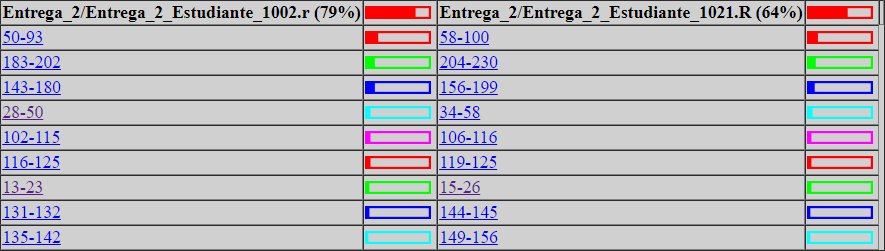
\includegraphics[scale=0.5]{imagenes/entrega2_MOSS_tabla.png}  %el parámetro scale permite agrandar o achicar la imagen. En el nombre de archivo puede especificar directorios
\caption{Tabla comparativa entre dos estudiantes en la segunda entrega con matlab como opción (MOSS)} \label{fig:entrega2_MOSS_2}
\end{figure}


\begin{figure}[] %con el [H] le obligamos a situar aquí la figura
\centering
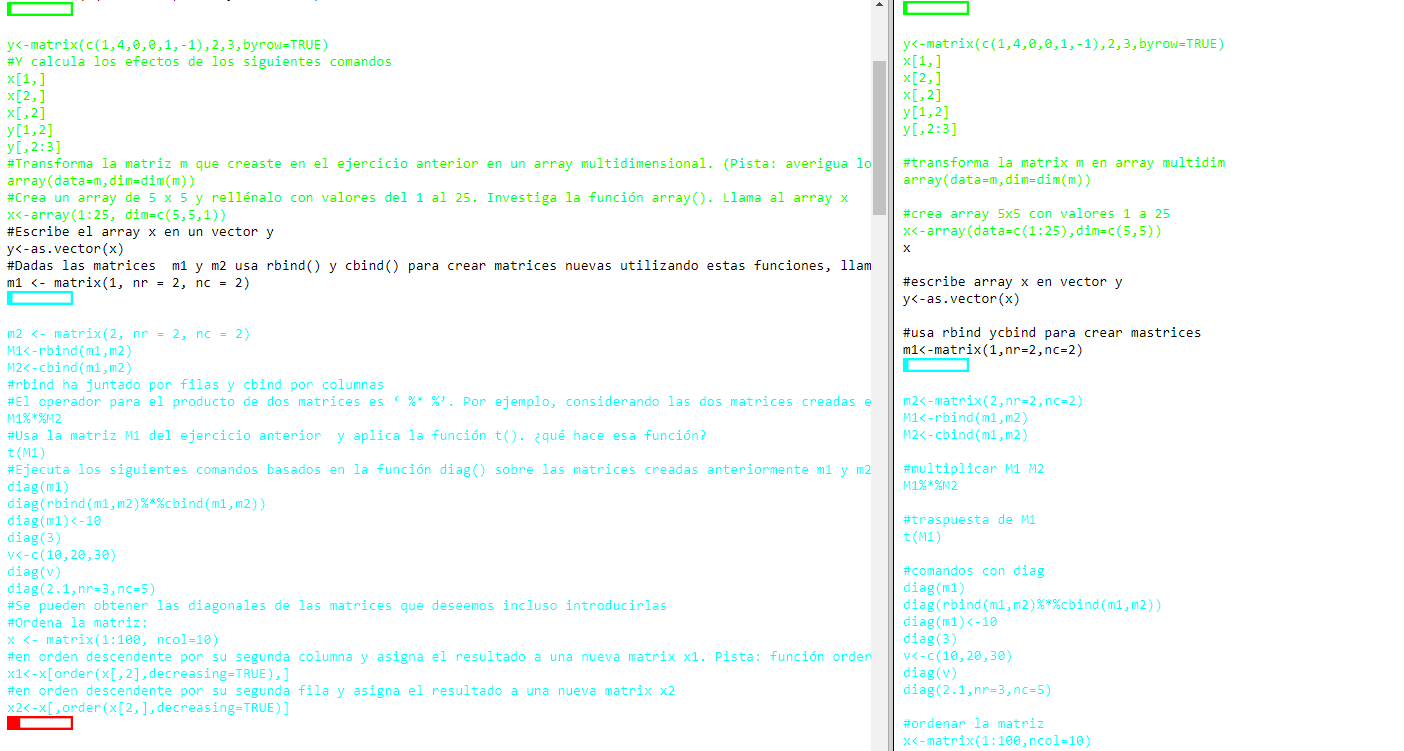
\includegraphics[width=14cm, height=10cm]{imagenes/entrega2_MOSS_comp.png}  %el parámetro scale permite agrandar o achicar la imagen. En el nombre de archivo puede especificar directorios
\caption{Parte comparativa del código fuente de dos estudiantes en la segunda entrega con matlab como opción (MOSS)} \label{fig:entrega2_MOSS_3}
\end{figure}


En la tabla de Figura \ref{fig:entrega2_MOSS_2} se muestra un rango con el número de líneas de cada archivo donde se considera que ha habido copia, junto con un ''termómetro'' para mostrar gráficamente cómo de grande es este fragmento en comparación con el archivo completo.
Estos ''termómetros'' así mismo son links que te situan en la parte del código al que se refieren en los otros dos marcos (Figura \ref{fig:entrega2_MOSS_3}).

\bigskip
\section{Ejecución en JPLAG}

Para usar JPLAG tendremos que descargar el código fuente completo de \cite{jplag_github}. Para usar nuestra versión con nuestro frontend de R podemos descargar el código de https://github.com/AntonioJavierRP/jplag.
\newline
Una vez hecho esto nos situamos con nuestra terminal en la carpeta principal, es decir, la que contiene todos los frontends. Para generar los ejecutables de cada frontend ejecutaremos la orden:
\begin{center}
\begin{lstlisting}[language=bash]
$ mvn clean generate-sources package
\end{lstlisting}
\end{center}
En caso de querer generar un único ejecutable usaremos la siguiente orden dentro de la carpeta jplag:
\begin{center}
\begin{lstlisting}[language=bash]
$ mvn clean generate-sources assembly:assembly
\end{lstlisting}
\end{center}
Para ejecutar cualquiera de las dos últimas ordenes es necesario tener instalado Apache Maven, las instrucciones de su instalación se encuentran en \cite{instalacion_maven}
\newline
Los ejecutables creados estarán en sus respectivas carpetas ''target'', en el caso de tener un único ejecutable este estará en jplag/target.
\newline

\subsection{Obtención de resultados}

En nuestro caso hemos llamado a JPLAG con las siguientes opciones (situándonos en jplag/target):

\begin{center}
\begin{lstlisting}[language=bash]
$ java -jar jplag-2.11.9-SNAPSHOT-jar-with-dependencies.jar -l R -r ../resultados/Entrega_X/ -s <ruta_directorio_entrega_X>
\end{lstlisting}
\end{center}

Se ha ejecutado esta orden para siete entregas distintas, con unos 30 archivos por entrega, dos veces, una para R y otra para texto plano.
\newline
Como se puede apreciar se ha usado la opción -l para especificar el lenguaje, -r para especificar donde guardar los resultados y -s para especificar la ruta donde se encuentran todos los archivos que se quieren evaluar.
Podemos visualizar el resto de opciones disponibles con su descripción ejecutando el .jar sin opciones:
\begin{center}
\begin{lstlisting}[language=bash]
$ java -jar jplag-2.11.9-SNAPSHOT-jar-with-dependencies.jar
\end{lstlisting}
\end{center}

Los resultados serán visualizables en el navegador, podemos abrir el archivo index.html para situarnos en la página principal de análisis de los resultados (Figuras \ref{fig:entrega2_JPLAG_1} y \ref{fig:entrega2_JPLAG_2}).
La interpretacion de estos resultados es muy similar a la que explicamos en apartados anteriores con MOSS, ya que su interfaz es muy similar.
\newline
A continuación explicamos cómo interpretar los elementos de la página principal de JPLAG.
\begin{figure}[t] %con el [H] le obligamos a situar aquí la figura
\centering
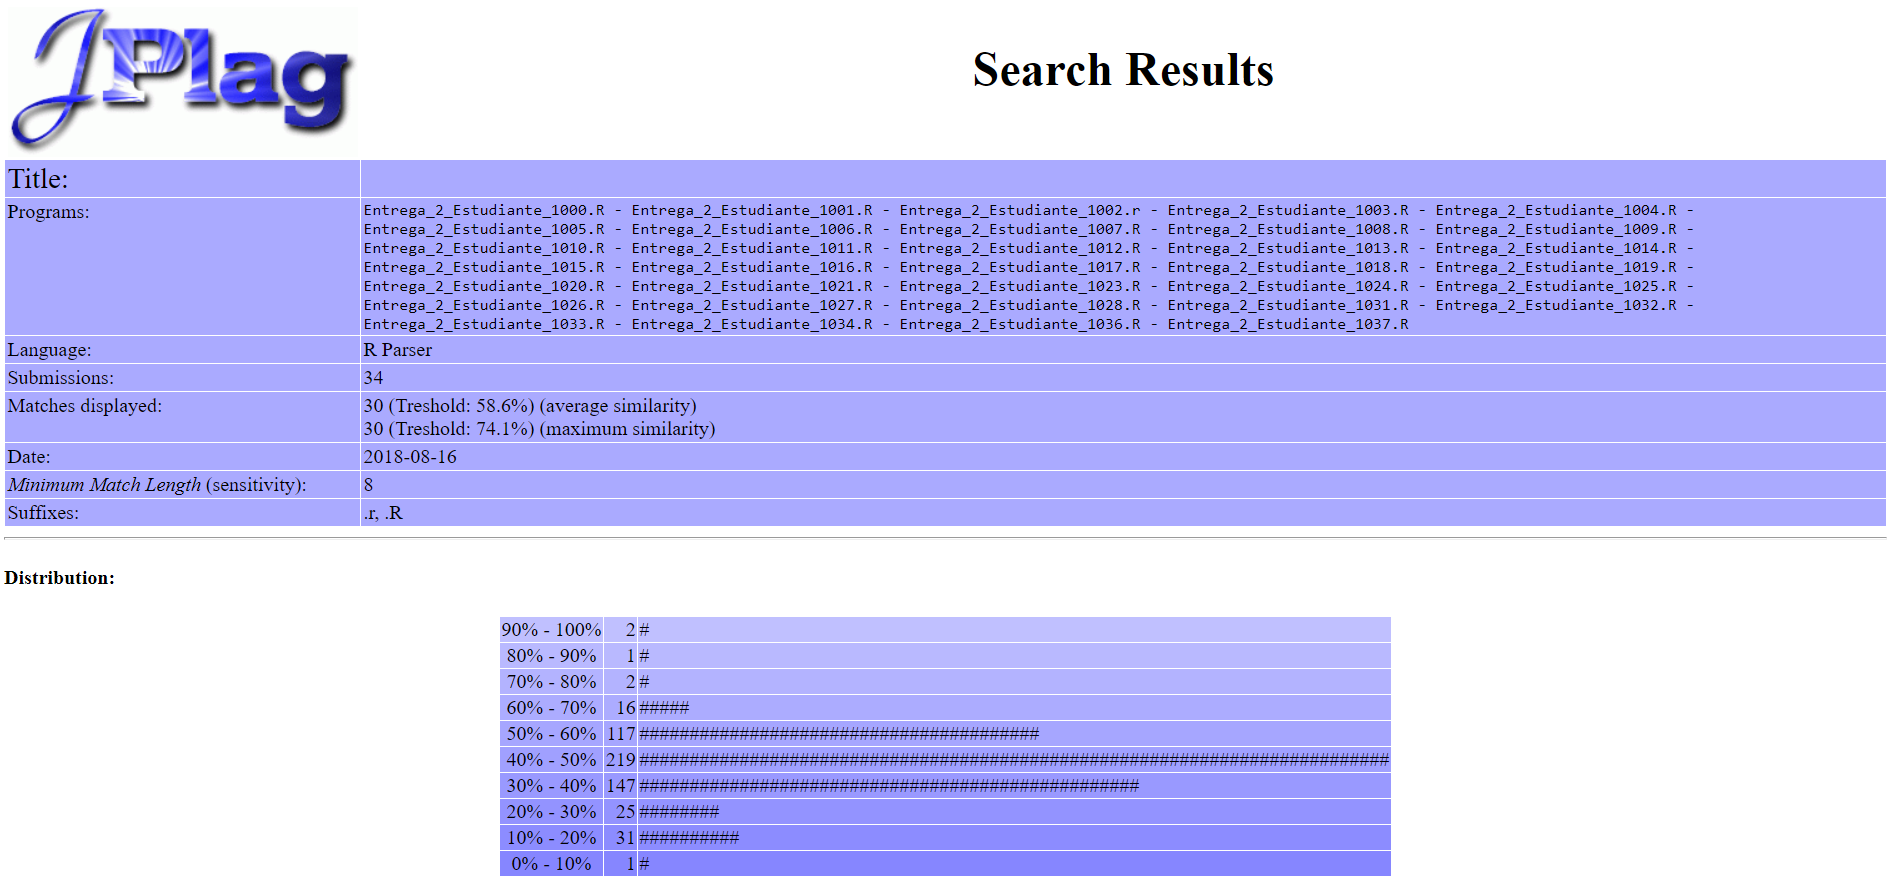
\includegraphics[width=14cm, height=9cm]{imagenes/entrega2_JPLAG_1.png}  %el parámetro scale permite agrandar o achicar la imagen. En el nombre de archivo puede especificar directorios
\caption{Página principal de los resultados de la Entrega 2 (JPLAG) parte 1} \label{fig:entrega2_JPLAG_1}
\end{figure}

\begin{figure}[t] %con el [H] le obligamos a situar aquí la figura
\centering
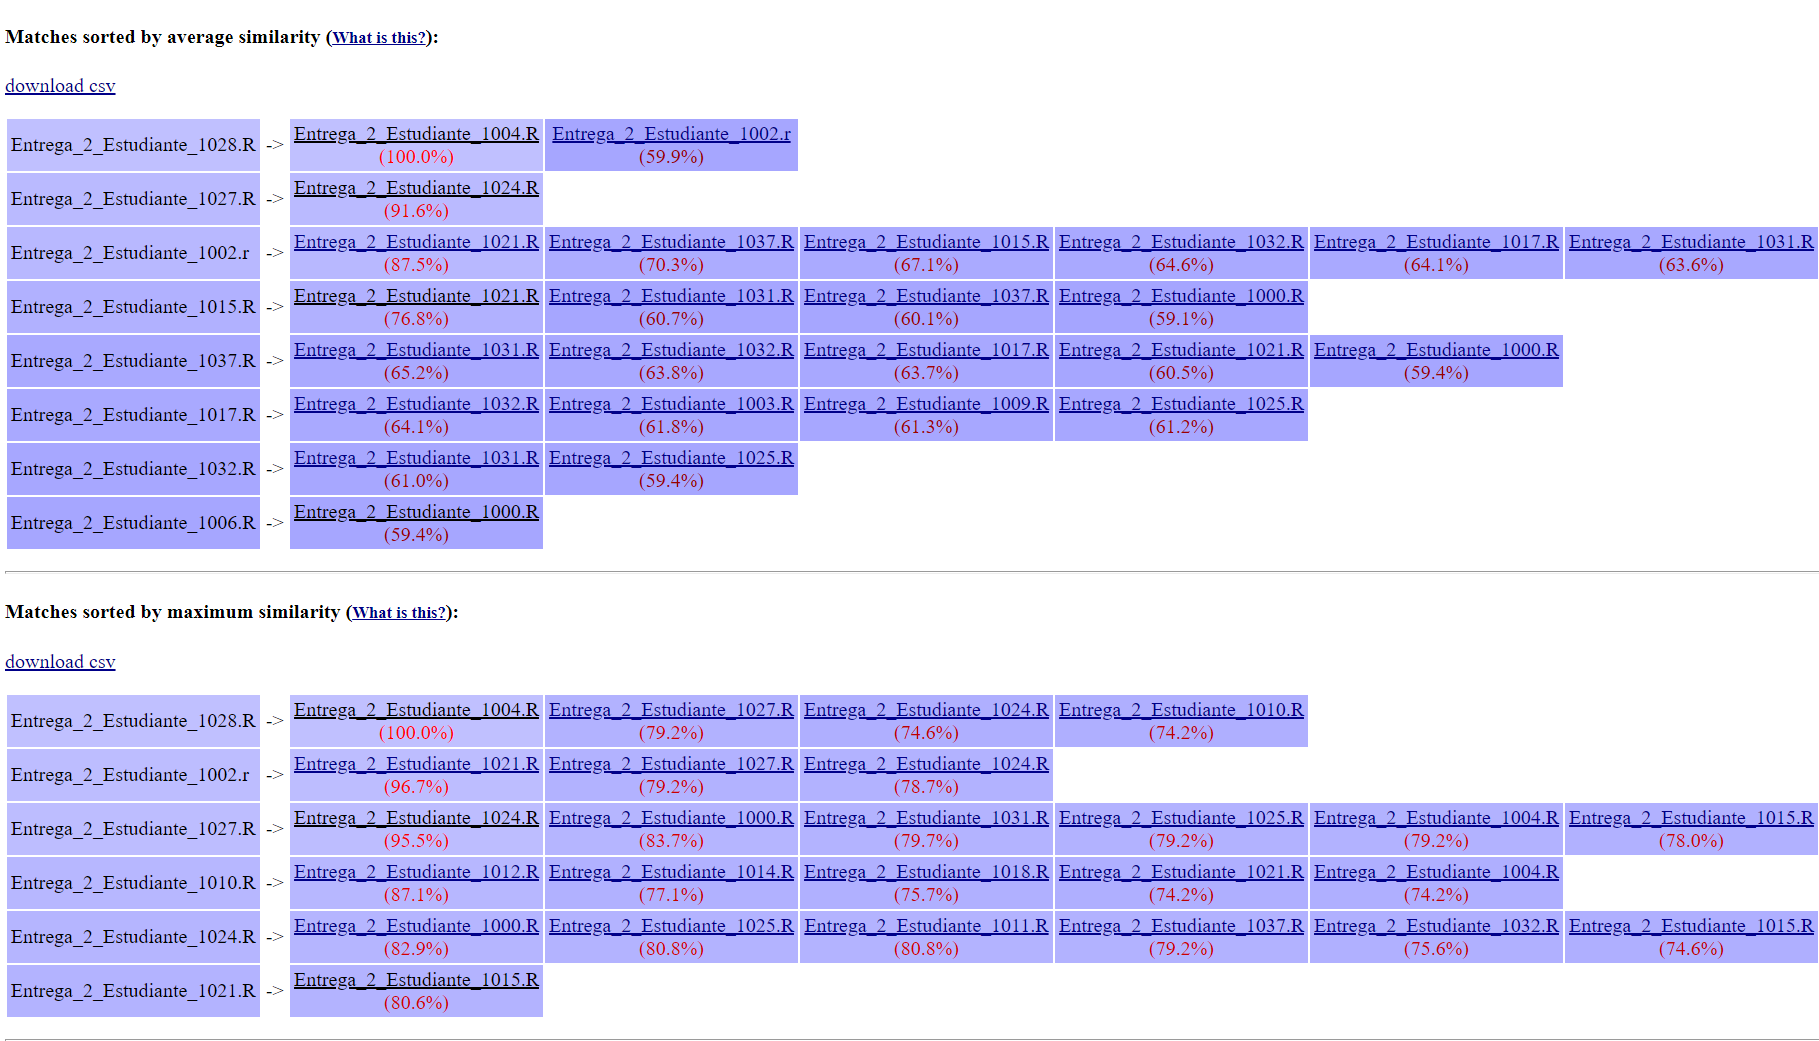
\includegraphics[width=14cm, height=9cm]{imagenes/entrega2_JPLAG_2.png}  %el parámetro scale permite agrandar o achicar la imagen. En el nombre de archivo puede especificar directorios
\caption{Página principal de los resultados de la Entrega 2 (JPLAG) parte 2} \label{fig:entrega2_JPLAG_2}
\end{figure}
La Figura \ref{fig:entrega2_JPLAG_1} contiene la parte de arriba de la página de resultados de la segunda entrega de los alumnos obtenida por nuestro frontend de R.
Se lista en una tabla el nombre de los programas que se han detectado, el idioma del parser usado, el número de archivos totales, el número de archivos emparejados que se muestran, la fecha en la que se obtuvieron los resultados, el número mínimo de tokens iguales que tiene que haber para que se considere un emparejamiento y las extensiones de los archivos procesados.
\newline
Seguido de esto, JPLAG muestra un histograma de los valores de similaridad encontrados en todos los pares de programas.
\newline
Podemos usar este histograma para identificar los casos que son plagio obvio y los que no tienen nada en común.
\newline
Los pares que se encuentran entre estos dos lados del espectro se encuentran a continuación en la parte de abajo de la página en Figura \ref{fig:entrega2_JPLAG_2}.
\newline
Se muestran ordenados en base a dos criterios, basándose en la cobertura entre programas (es decir, cuánto de un programa se ha usado en otro):
\begin{itemize}
\item Similaridad Media: media entre las coberturas de ambos programas entre si. Emparejamientos con una alta cobertura indican pares muy similares.
\item Similaridad Máxima: el máximo entre las dos coberturas. Esta medida es útil para encontrar los casos en los que ha habido plagio y se ha añadido código extra para ''rellenar'' y que los archivos tengan tamaños muy diferentes.
\end{itemize}

Haciendo click en el nombre de alguno de estos archivos iremos a la página comparativa de código entre estos.
\newline
En la parte superior de la página (Figura \ref{fig:entrega2_JPLAG_3}) tenemos a la izquierda el nombre de los archivos que se comparan, su porcentaje de similaridad y dos hiperlinks uno para volver a la página principal y otro de ayuda. A la derecha de esta página se muestra una tabla similar a la que teníamos en MOSS, en la que también se listan los trozos de código donde se han encontrado cadenas de tokens idénticas. Por cada par de trozos de código se especifica el número de tokens en común que se han encontrado seguidos y el color que se le ha asignado para que su visualización sea más facil en la parte de abajo de esta misma página (Figura \ref{fig:entrega2_JPLAG_4}).
\newline
En esta parte cada pasaje encontrado tiene una especie de flecha al principio, al pinchar sobre esta se alinea la otra parte del código del otro programa para que se puedan ver lado a lado los trozos de código con el mismo color.
Si una parte del código no coincide con la del otro programa esta se mostrará en color negro.


\begin{figure}[H] %con el [H] le obligamos a situar aquí la figura
\centering
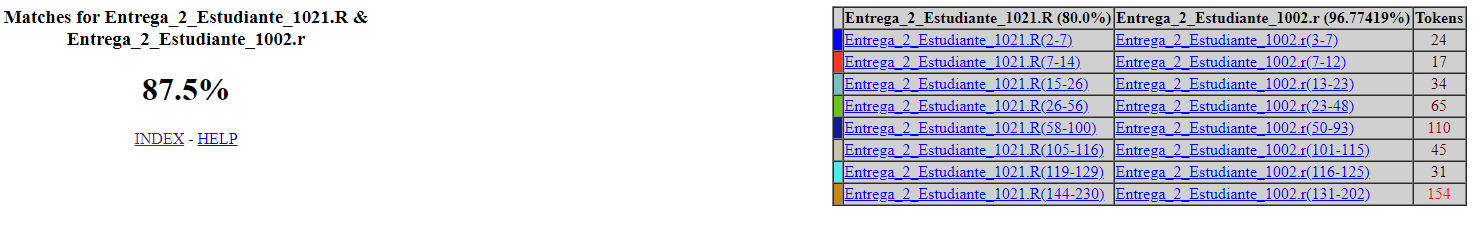
\includegraphics[scale=0.3]{imagenes/entrega2_JPLAG_3.png}  %el parámetro scale permite agrandar o achicar la imagen. En el nombre de archivo puede especificar directorios
\caption{Página de comparación de código entre dos archivos en JPLAG (parte de arriba)} \label{fig:entrega2_JPLAG_3}
\end{figure}


\begin{figure}[H] %con el [H] le obligamos a situar aquí la figura
\centering
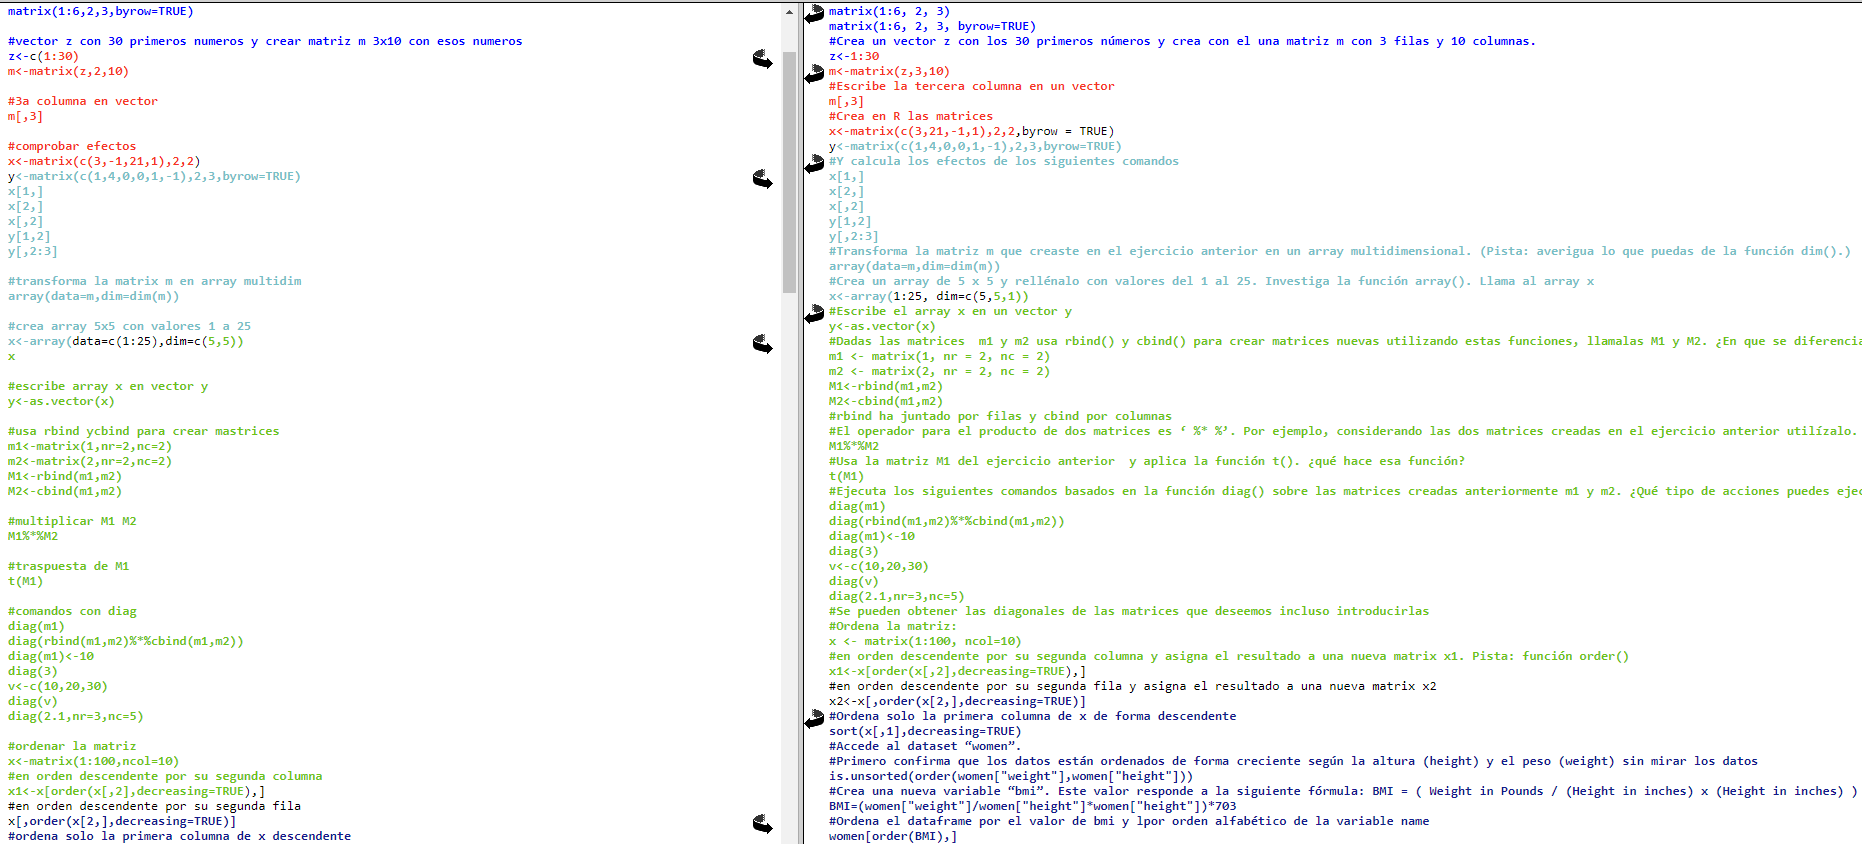
\includegraphics[width=14cm, height=9cm]{imagenes/entrega2_JPLAG_4.png}  %el parámetro scale permite agrandar o achicar la imagen. En el nombre de archivo puede especificar directorios
\caption{Página de comparación de código entre dos archivos en JPLAG (parte de abajo)} \label{fig:entrega2_JPLAG_4}
\end{figure}

\section{Pruebas}

Para comprobar que el frontend que hemos creado facilita la detección de plagio entre archivos en R, se ha hecho un estudio de las diferencias entre los resultados obtenidos con nuestra versión de JPLAG usando el frontend de R y los resultados que se podían obtener usando otros medios ya existentes.
\newline
Los archivos en R usados para realizar este estudio han sido las entregas de los alumnos de la asignatura ''Introducción a la programación para ciencia de datos'' del Master de ciencia de datos de la Universidad de Granada.
\newline
Cada entrega consiste en ejercicios sobre diferentes aspectos de R, empezando por una introducción con ejercicios simples y añadiendo nuevos conceptos y estructuras de R con cada nueva entrega.
\newline
Son un total de 7 entregas:
\begin{itemize}
\item \textbf{Entrega 1.} Introducción a R y ejercicios de vectores. 36 programas enviados(cada programa es un archivo de un único alumno).
\item \textbf{Entrega 2.} Ejercicios de matrices, arrays y factores. 34 programas enviados.
\item \textbf{Entrega 3.} Ejercicios de manipulación de strings. 36 programas enviados.
\item \textbf{Entrega 4.} Ejercicios de dataframes y listas. 33 programas enviados.
\item \textbf{Entrega 5.} Ejercicios de entrada y salida. 36 programas enviados.
\item \textbf{Entrega 6.} Ejercicios de Funciones. 36 programas enviados.
\item \textbf{Entrega 7.} Ejercicios de estructuras de programación en R. 36 programas enviados.
\end{itemize}
Los ejercicios de los alumnos se han convertido a archivos .R (ya que en algunos archivos estaban en .pdf, .docx, .rmd,...) para que JPLAG los pueda procesar y han sido ademas anonimizados asignándosele a cada alumno un ID. Hay 38 alumnos en total.
\newline
Cada una de estas entregas ha sido procesada en JPLAG con nuestro frontend, con el frontend de texto plano y en MOSS en modo Matlab y texto plano.

Se han analizado los resultados en base a las entregas:
\subsection{Análisis de resultados}

Se han analizado los resultados en base a las peculiaridades de cada entrega, ya que estas se dividen en diferentes aspectos del lenguaje, lo cual es idóneo para observar la precisión de la detección de plagio en ejercicios de áreas totalmente distintas.

\bigskip


La primera entrega consiste en una serie de ejercicios de introducción a R, para que el alumno aprenda cómo generar secuencias de números, usar vectores y a usar las llamadas más comunes que se usan en R.
\newline
Por norma general los alumnos han necesitado aproximadamente cien líneas de código para completar estos ejercicios, aunque los programas tienen más de doscientas en total debido a comentarios con aclaraciones sobre el código y con los enunciados de los ejercicios.
\newline
Los resultados obtenidos en esta entrega con JPLAG se pueden ver plasmados en dos histogramas en Figura \ref{fig:histograma1} donde se muestran los valores de similaridad media para todos los pares posibles de programas (en esta entrega al ser 36 programas habrá 630 emparejamientos diferentes).


\begin{figure}[H] %con el [H] le obligamos a situar aquí la figura
\centering
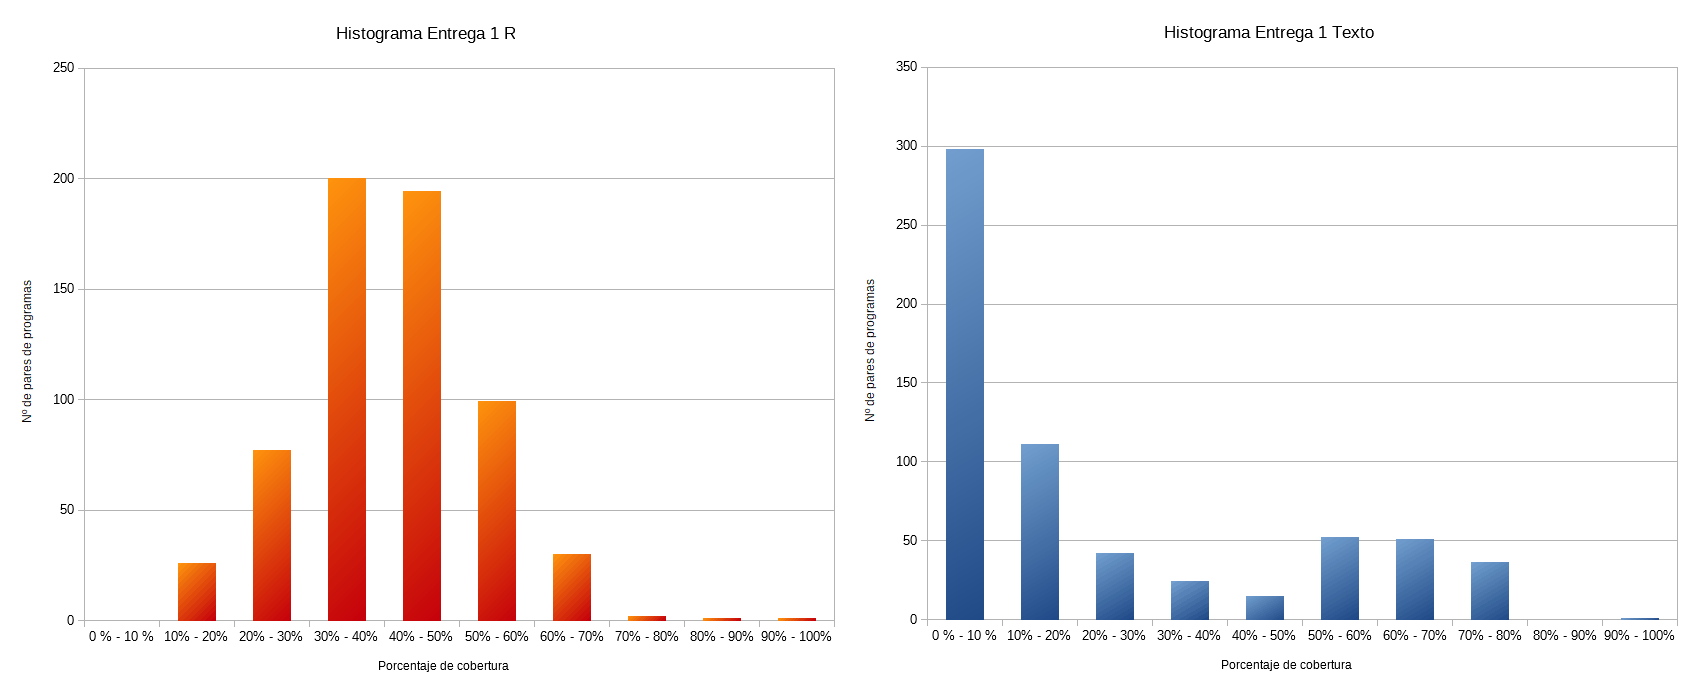
\includegraphics[width=15cm, height=7cm]{imagenes/histograma1.png}  %el parámetro scale permite agrandar o achicar la imagen. En el nombre de archivo puede especificar directorios
\caption{Histogramas de valores de similaridad entre todos los pares de programas de la primera entrega.} \label{fig:histograma1}
\end{figure}



Para evitar mostrar este caso repetidas veces con cada gráfica que se muestre, se ha de mencionar que en todas las entregas hechas menos en la séptima, los estudiantes con id 1004 y 1028 se han copiado al 100\%, es decir, han entregado programas iguales.
\newline
\bigskip

Como era de esperar, el frontend de JPLAG de texto plano, correspondiente al histograma de la derecha, sólo detecta plagio en caso de que se haya hecho una copia literal del código, es decir, que sea exáctamente el mismo con las mismas palabras. Por esta razón la mayor parte de los pares de programas tienen un índice de cobertura (o similaridad) muy bajo. Existen algunos casos con un índice alto, pero esto se debe a similaridad en los comentarios, ya que algunos alumnos han escrito en los comentarios del programa el enunciado de los ejercicios o explicaciones similares.
\newline
En el caso de nuestro frontend de R (histograma a la izquierda), se detectan una gran cantidad de pares con un índice de cobertura superior al treinta porciento, esto se debe a que los ejercicios de esta entrega son muy concretos y no hay muchas formas de hacerlos por lo que es normal que los alumnos hayan usado estructuras muy similares que al fin y al cabo están formadas por los mismos tokens.
\newline
Los pares con un índice superior al 70 porciento son casos casi seguros de plagio ya que es altamente improbable que dos alumnos tengan más de un setenta porciento de su código estructuralmente igual en 100 líneas de código sin haberse copiado.
\newline
En las gráficas de Figura \ref{fig:TOP10_1} podemos ver una representación de los resultados obtenidos en MOSS.
\newline 
En estas gráficas figuran los índices de similaridad de los 10 pares de programas más ''parecidos'' de la primera entrega. 


\begin{figure}[H] %con el [H] le obligamos a situar aquí la figura
\centering
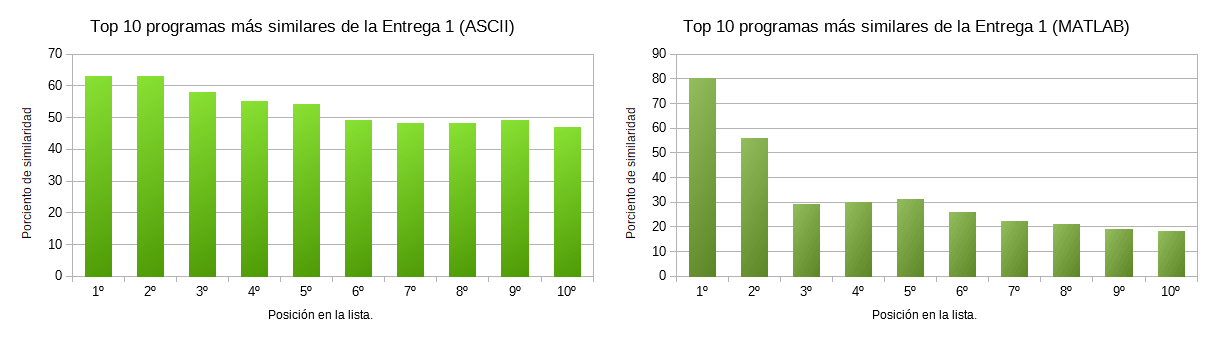
\includegraphics[width=14cm, height=6cm]{imagenes/TOP10_1.png}  %el parámetro scale permite agrandar o achicar la imagen. En el nombre de archivo puede especificar directorios
\caption{10 primeros pares de programas con mayor cantidad de código en común de la entrega 1} \label{fig:TOP10_1}
\end{figure}


Se puede apreciar que estos índices son más bajos que los obtenidos en JPLAG, esto en parte es debido a que MOSS ignora fragmentos de código que se repiten en al menos diez programas, lo que permite lidiar en cierta forma con los comentarios con el enunciado de los ejercicios (si es que al menos diez alumnos han decidido ponerlos).
\newline
Aun así, los resultados en modo texto plano (ASCII) sólo nos ayudan a encontrar programas con comentarios iguales o con código idéntico.
\newline
MOSS no encuentra tantas ocurrencias de plagio como nuestra versión de JPLAG, ya que se basa en un algoritmo que no tiene en cuenta los tokens si no un vector de características.
\newline
Lo que hace MOSS es tener en cuenta las palabras comunes del lenguaje elegido y en caso de aparecer no las considera plagio y no las tiene en cuenta en los índices de similaridad.
\newline
Los resultados obtenidos eligiendo como opción Matlab (ya que es el lenguaje mas parecido a R de los compatibles) son mejores que los de texto plano ya que nos han permitido encontrar algunas partes con sintaxis idéntica entre programas. De todas formas nuestro frontend de R ha encontrado estas mismas similaridades sintácticas además de una gran cantidad de plagio estructural y plagio en el que se cambia de orden el código o se añade código muerto, como en el caso de la Figura  \ref{fig:ENTREGA1_ESTRUCTURAL}, donde se ha encontrado un fragmento muy similar entre el código de los alumnos 1002 y 1036 que el resto de herramientas no ha detectado.

\bigskip
\begin{figure}[H] %con el [H] le obligamos a situar aquí la figura
\centering
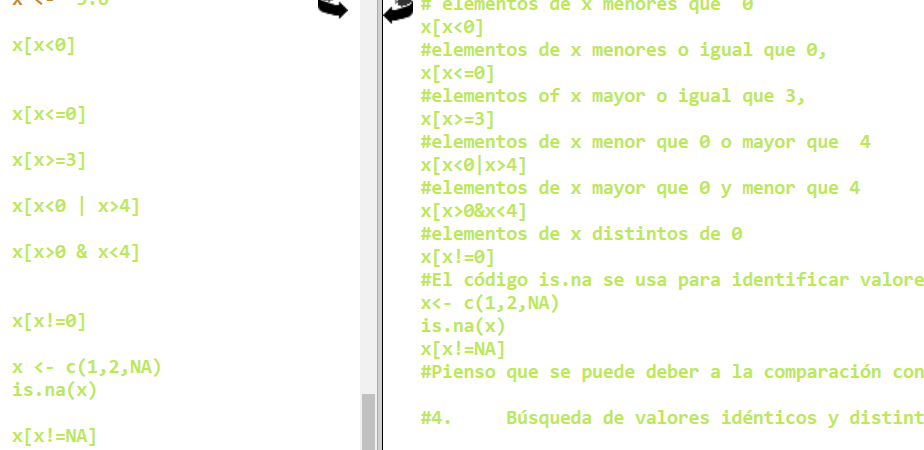
\includegraphics[width=8cm, height=5cm]{imagenes/ENTREGA1_ESTRUCTURAL.png}  %el parámetro scale permite agrandar o achicar la imagen. En el nombre de archivo puede especificar directorios
\caption{Ejemplo de plagio que sólo nuestro frontend ha encontrado en la primera entrega} \label{fig:ENTREGA1_ESTRUCTURAL}
\end{figure}

\bigskip
\bigskip


Las entregas 2 y 4 son muy similares ya que contienen ejercicios de uso de matrices, manipular y mostrar los datos que queramos de un dataset y manejo de factores(sólo en la 2), listas (sólo en la 4)y dataframes (sólo en la 4).
\newline
Ambas entregas son más del doble de largas que la primera entrega.
\newline

A continuación mostramos lás gráficas de los resultados para estas entregas (Figuras \ref{fig:histograma2}, \ref{fig:TOP10_2},\ref{fig:histograma4}, \ref{fig:TOP10_4}):

\begin{figure}[H] %con el [H] le obligamos a situar aquí la figura
\centering
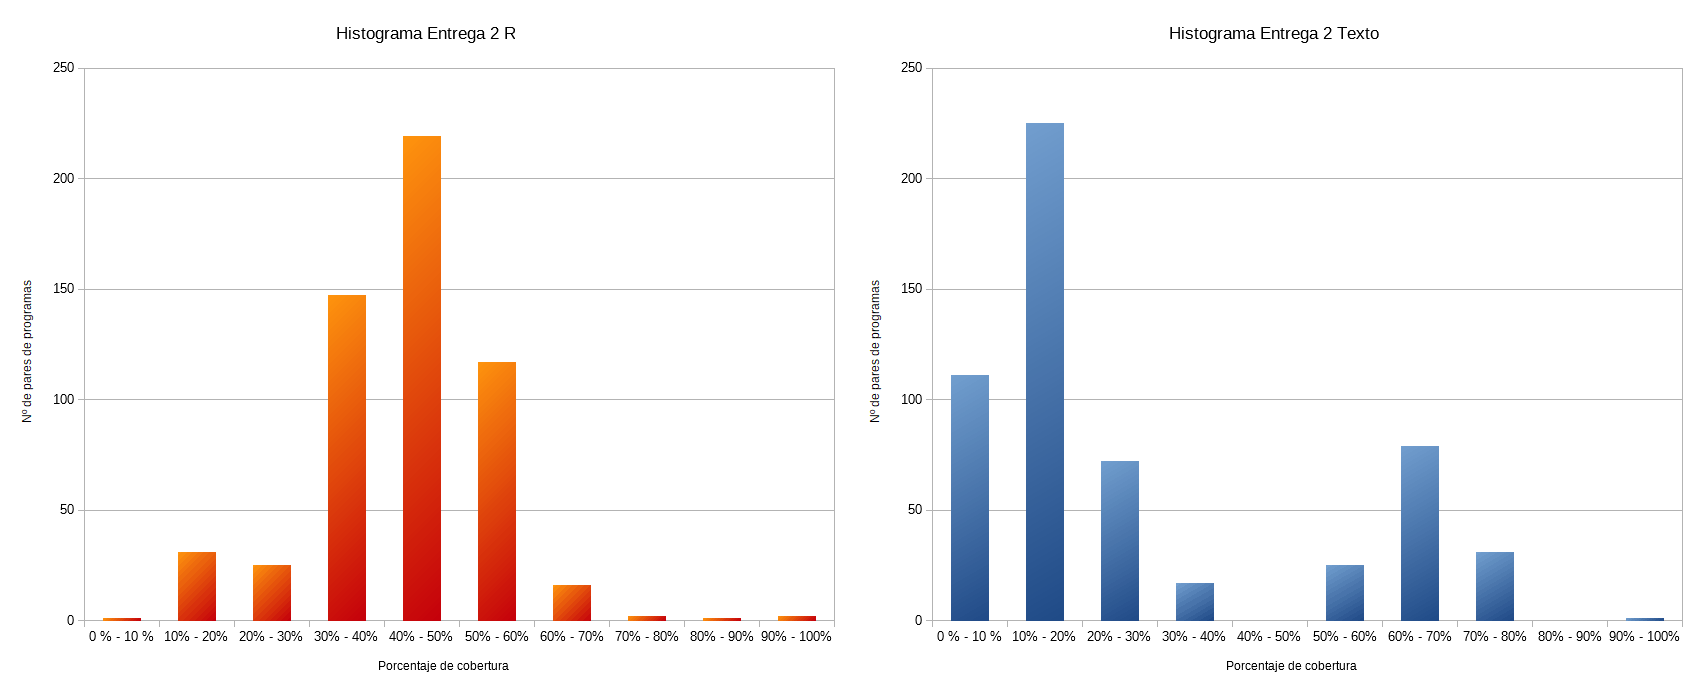
\includegraphics[width=15cm, height=7cm]{imagenes/histograma2.png}  %el parámetro scale permite agrandar o achicar la imagen. En el nombre de archivo puede especificar directorios
\caption{Histogramas de valores de similaridad entre todos los pares de programas de la segunda entrega.} \label{fig:histograma2}
\end{figure}


\begin{figure}[H] %con el [H] le obligamos a situar aquí la figura
\centering
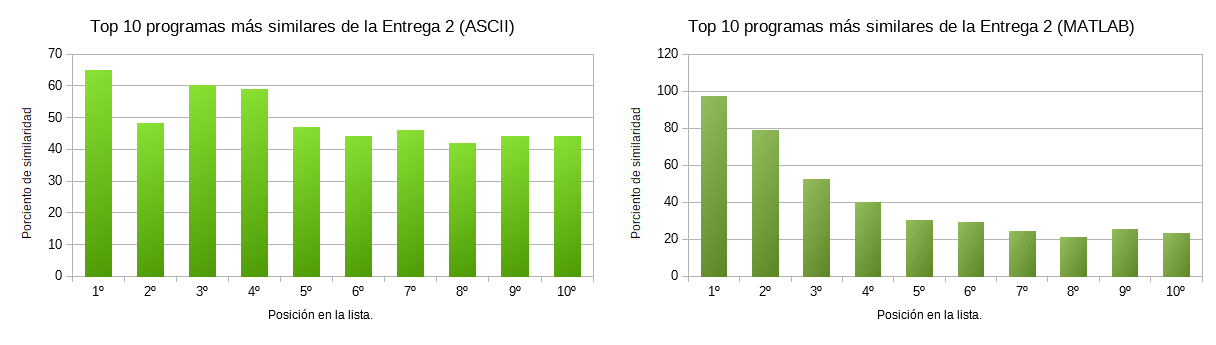
\includegraphics[width=14cm, height=6cm]{imagenes/TOP10_2.png}  %el parámetro scale permite agrandar o achicar la imagen. En el nombre de archivo puede especificar directorios
\caption{10 primeros pares de programas con mayor cantidad de código en común de la entrega 2} \label{fig:TOP10_2}
\end{figure}



\begin{figure}[H] %con el [H] le obligamos a situar aquí la figura
\centering
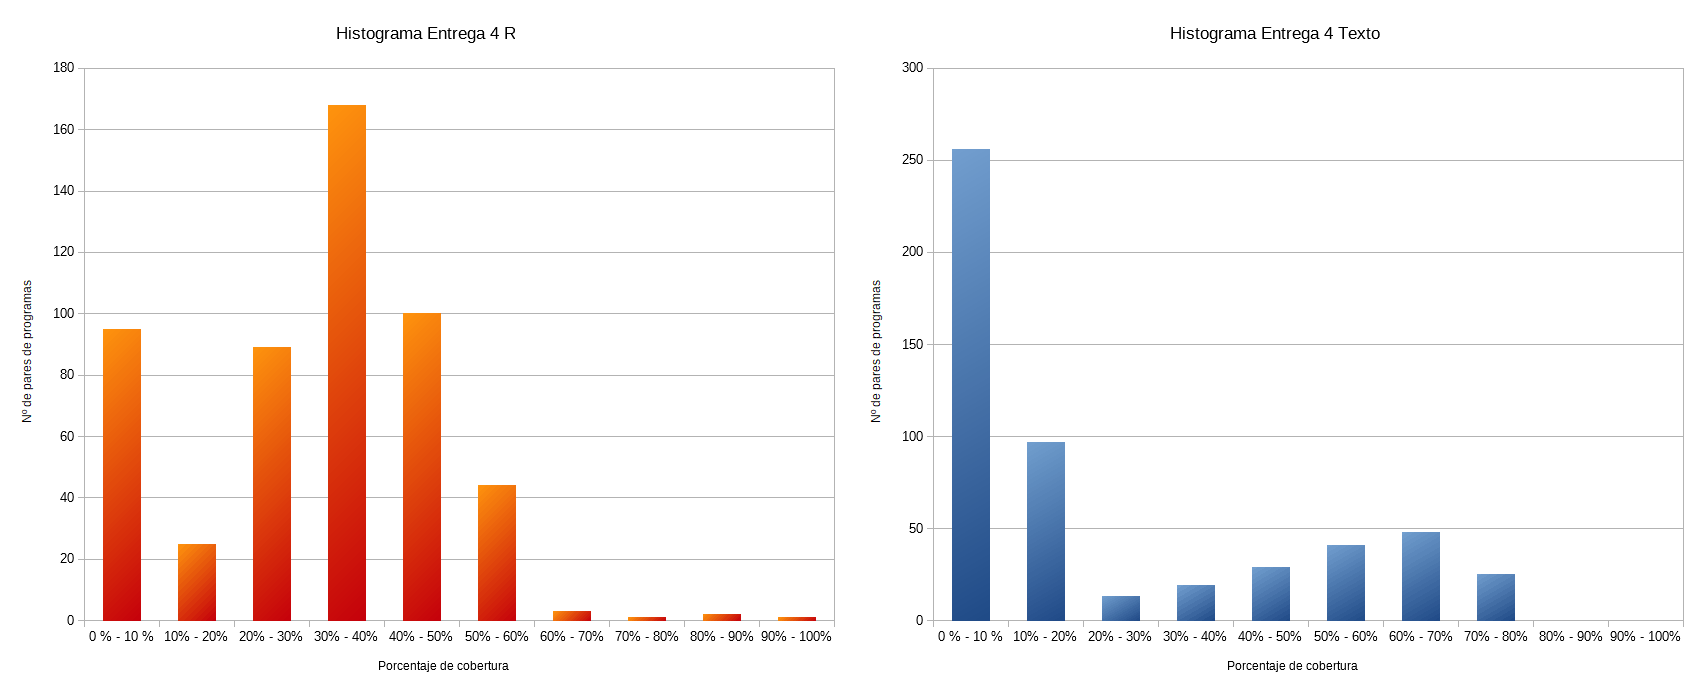
\includegraphics[width=15cm, height=7cm]{imagenes/histograma4.png}  %el parámetro scale permite agrandar o achicar la imagen. En el nombre de archivo puede especificar directorios
\caption{Histogramas de valores de similaridad entre todos los pares de programas de la cuarta entrega.} \label{fig:histograma4}
\end{figure}



\begin{figure}[H] %con el [H] le obligamos a situar aquí la figura
\centering
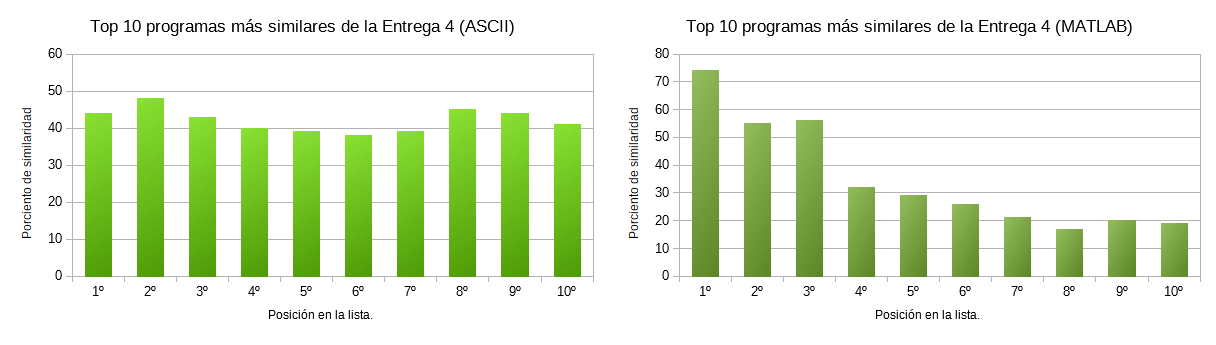
\includegraphics[width=14cm, height=6cm]{imagenes/TOP10_4.png}  %el parámetro scale permite agrandar o achicar la imagen. En el nombre de archivo puede especificar directorios
\caption{10 primeros pares de programas con mayor cantidad de código en común de la entrega 4} \label{fig:TOP10_4}
\end{figure}



Al consistir estas en programas más largos es más complicado que tengan una gran cantidad de código en común, es por esto que los histogramas de JPLAG y las gráficas de MOSS de estas entregas tienen índices de similaridad menores que los de la entrega 1.
\newline
Aún así JPLAG con nuestro frontend sigue encontrando bastantes pares con similaridad superior al 30\%. 

\bigskip
El resto de entregas son cortas pero obtenemos gráficas distintas debido a los ejercicios de cada una de estas:
\newline
La tercera y quinta entregas son algo distintas de lo visto hasta el momento, son entregas muy cortas con ejercicios similares; con 5 ejercicios de manipulación de strings en la tercera entrega y 5 ejercicios de E/S en la quinta.
\newline
Las gráficas de estas entregas se muestran a continuación(Figuras \ref{fig:histograma3}, \ref{fig:TOP10_3}, \ref{fig:histograma5}, \ref{fig:TOP10_5}):



\begin{figure}[H] %con el [H] le obligamos a situar aquí la figura
\centering
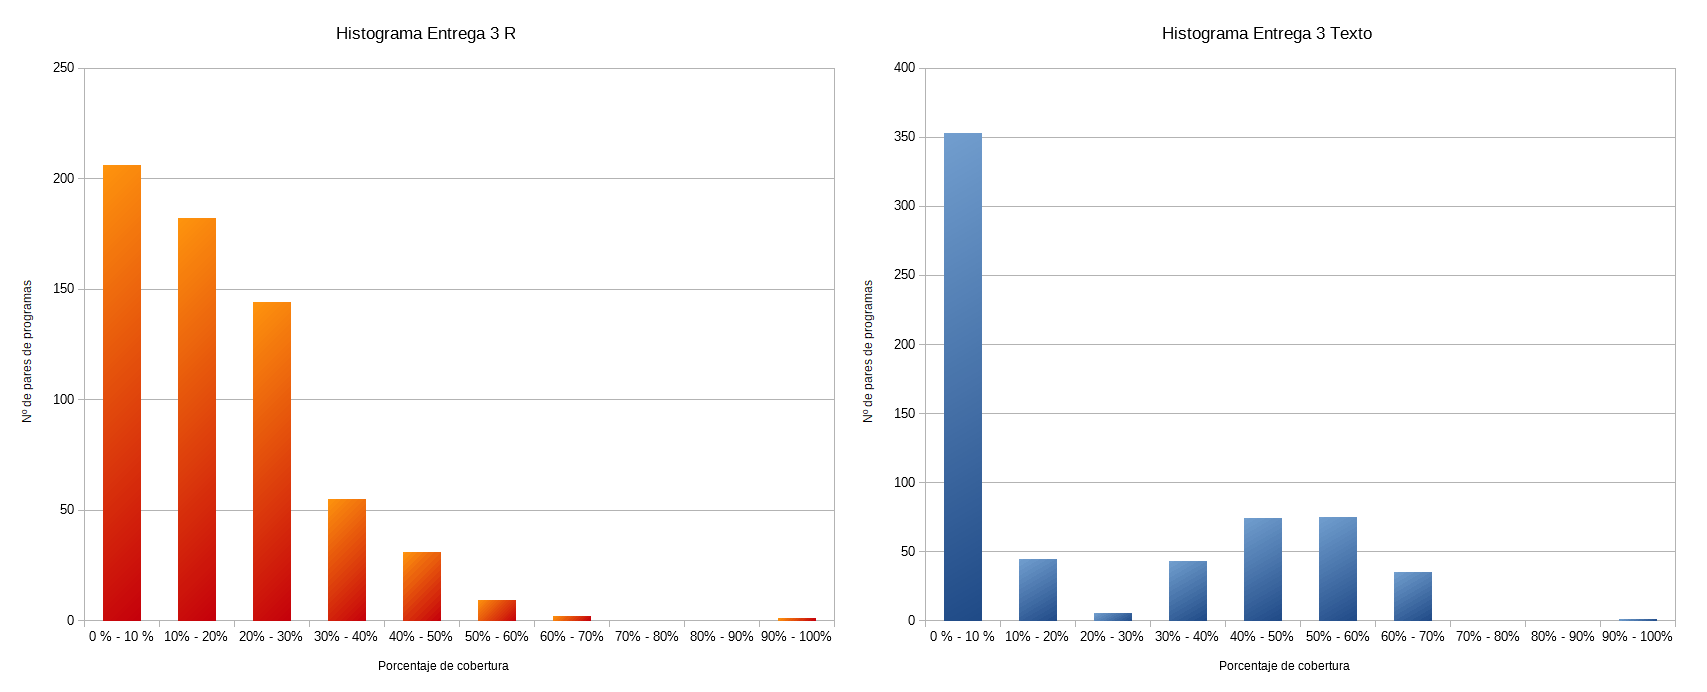
\includegraphics[width=15cm, height=7cm]{imagenes/histograma3.png}  %el parámetro scale permite agrandar o achicar la imagen. En el nombre de archivo puede especificar directorios
\caption{Histogramas de valores de similaridad entre todos los pares de programas de la tercera entrega.} \label{fig:histograma3}
\end{figure}


\begin{figure}[H] %con el [H] le obligamos a situar aquí la figura
\centering
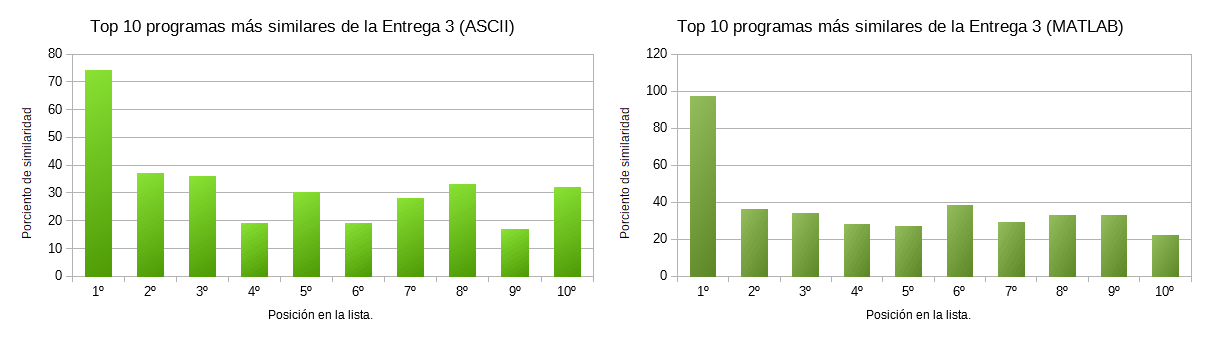
\includegraphics[width=14cm, height=6cm]{imagenes/TOP10_3.png}  %el parámetro scale permite agrandar o achicar la imagen. En el nombre de archivo puede especificar directorios
\caption{10 primeros pares de programas con mayor cantidad de código en común de la entrega 3} \label{fig:TOP10_3}
\end{figure}


\begin{figure}[H] %con el [H] le obligamos a situar aquí la figura
\centering
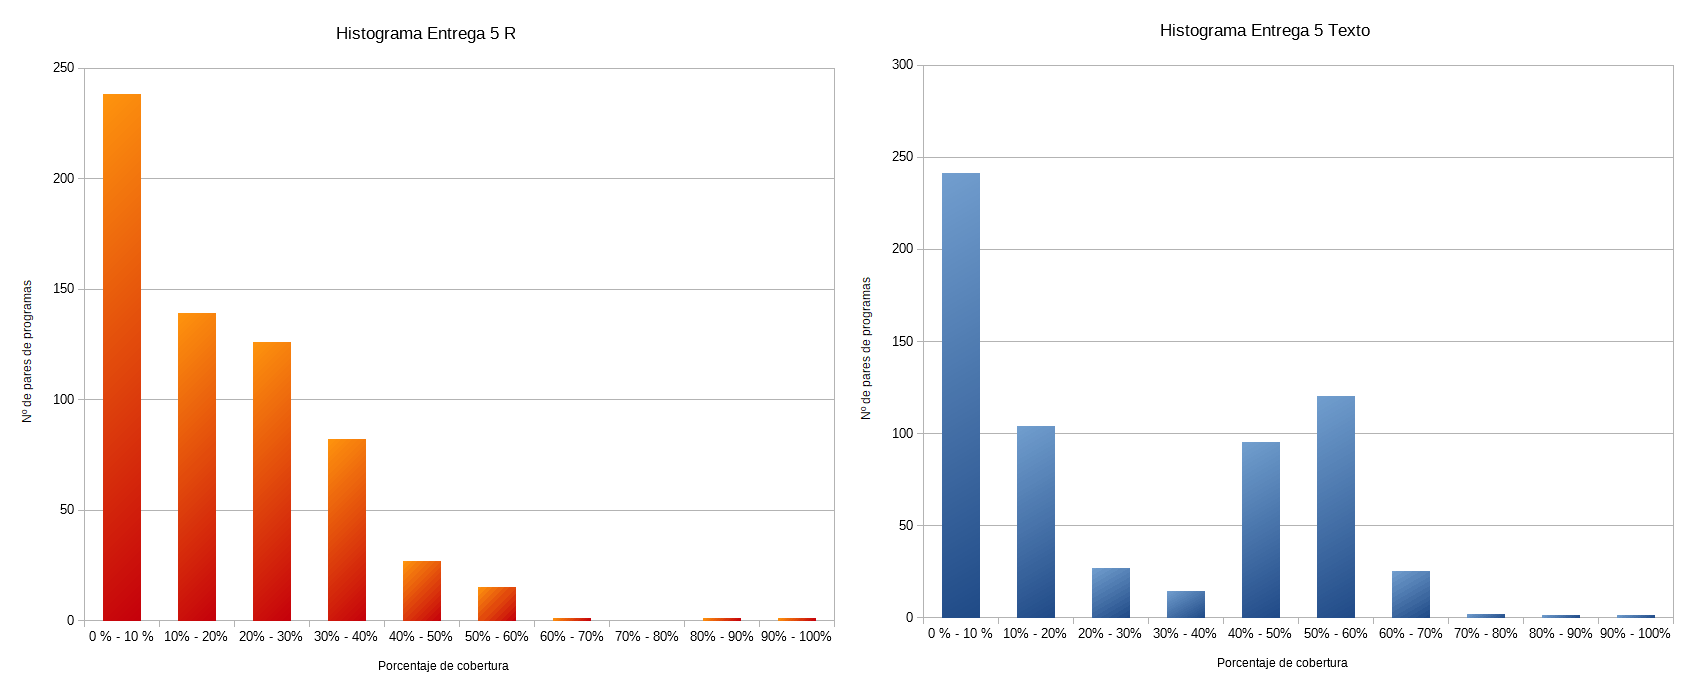
\includegraphics[width=15cm, height=7cm]{imagenes/histograma5.png}  %el parámetro scale permite agrandar o achicar la imagen. En el nombre de archivo puede especificar directorios
\caption{Histogramas de valores de similaridad entre todos los pares de programas de la quinta entrega.} \label{fig:histograma5}
\end{figure}





\begin{figure}[H] %con el [H] le obligamos a situar aquí la figura
\centering
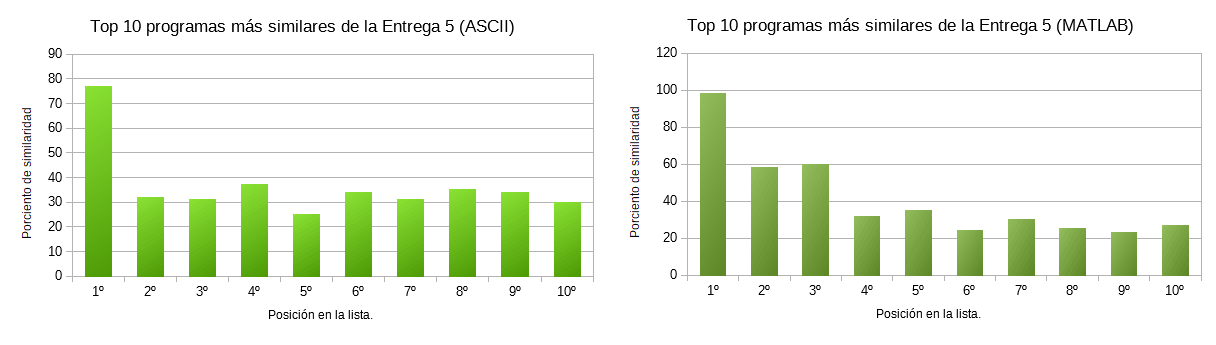
\includegraphics[width=14cm, height=6cm]{imagenes/TOP10_5.png}  %el parámetro scale permite agrandar o achicar la imagen. En el nombre de archivo puede especificar directorios
\caption{10 primeros pares de programas con mayor cantidad de código en común de la entrega 5} \label{fig:TOP10_5}
\end{figure}



Aún siendo ejercicios muy cortos los que se piden en estas entregas, estos se pueden abordar de numerosas formas, es por esto que los índices de similaridad detectados con JPLAG y MOSS entre estos pares de archivos son los más bajos hasta el momento.
\newline
Los pares detectados en MOSS y en JPLAG con texto con un índice superior al 40\% se deben a programas de alumnos que han escrito el enunciado de los ejercicios en su código, y al ser tan pocas las líneas de código que se requieren para hacerlo, los comentarios suponen más de un 50\% del documento en la mayoría de los casos.
\newline
Por otra parte, los contados casos en los que nuestro frontend ha detectado un alto porcentaje de cobertura entre emparejamientos se deben en su mayoría a alumnos que se han copiado pero han intentado ocultarlo cambiando el nombre de la variables, el de las cadenas de strings usadas y el de los documentos usados en los ejercicios de E/S.
Podemos ver un ejemplo de estos en Figura \ref{fig:ENTREGA5_variable}:


\begin{figure}[H] %con el [H] le obligamos a situar aquí la figura
\centering
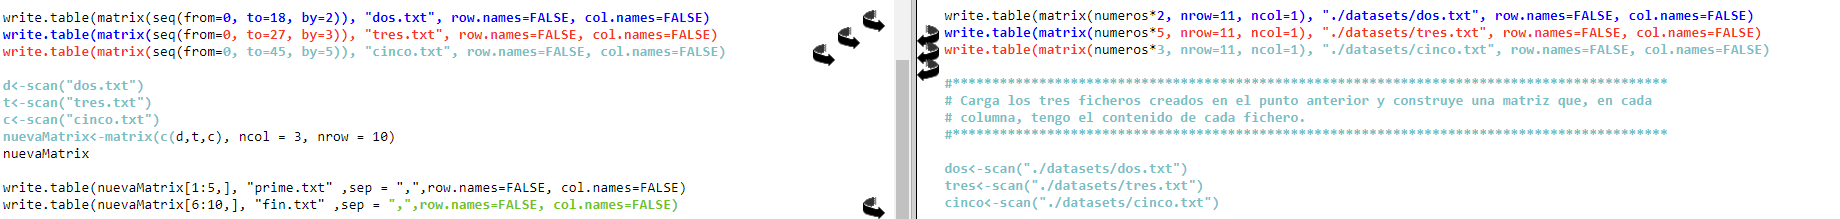
\includegraphics[width=15cm, height=5cm]{imagenes/ENTREGA5_variable.png}  %el parámetro scale permite agrandar o achicar la imagen. En el nombre de archivo puede especificar directorios
\caption{Ejemplo de plagio entre alumnos en el que se ha cambiado el nombre de variables y archivos(Entrega 5)} \label{fig:ENTREGA5_variable}
\end{figure}

\bigskip
Por último, en las entregas 6 y 7 se obtienen resultados similares a las entregas 3 y 5, ya que son igual de cortas, pero a diferencia de estas, tratan sobre ejercicios que requieren la definición de funciones. 
\newline
Para declarar una función como las que se piden en los ejercicios de estas entregas el alumno usará sus propias estructuras de control, variables y cálculos matemáticos.
\newline
Debido a esto se obtienen las siguientes gráficas de resultados (Figuras \ref{fig:histograma6}, \ref{fig:TOP10_6}, \ref{fig:histograma7}, \ref{fig:TOP10_7}):



\begin{figure}[H] %con el [H] le obligamos a situar aquí la figura
\centering
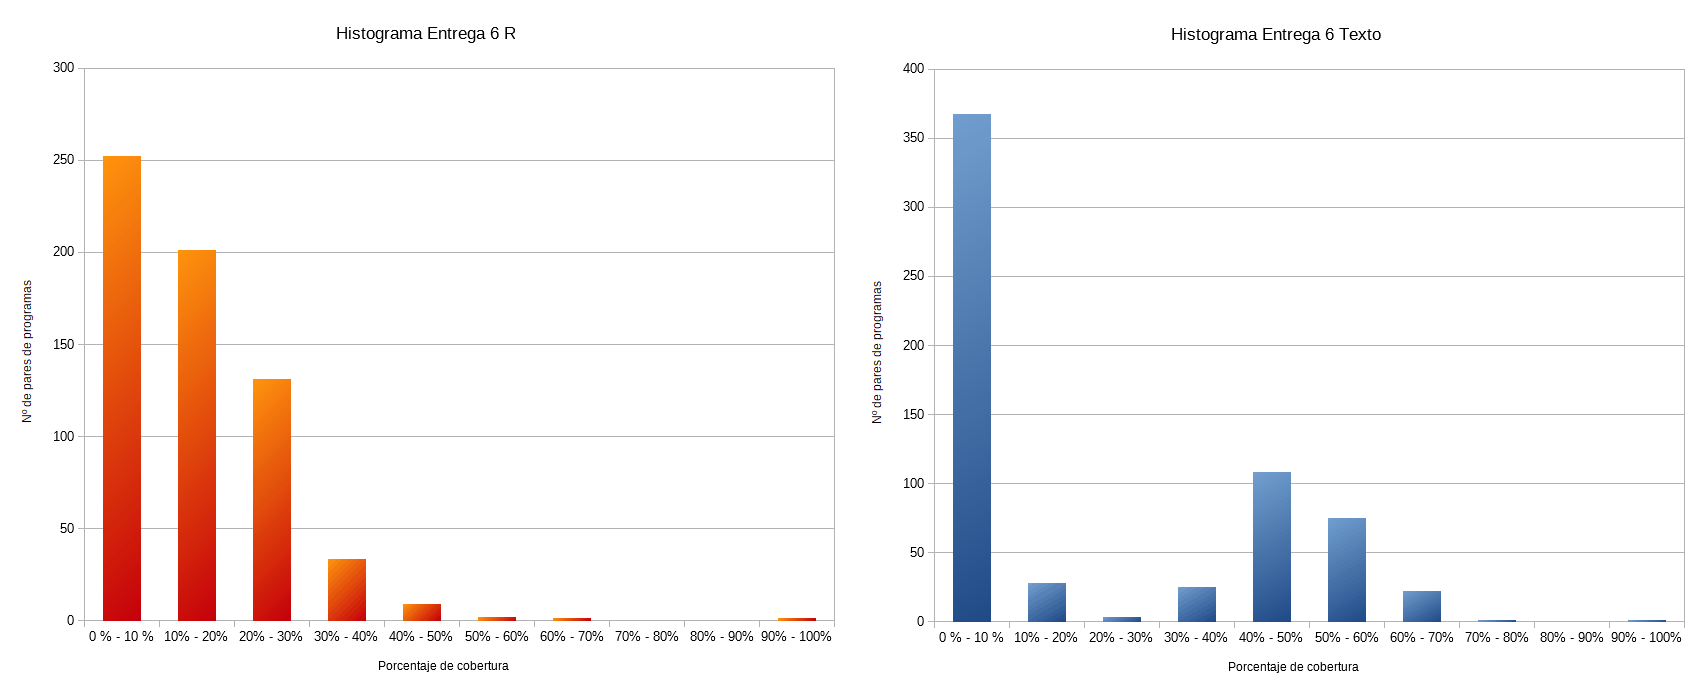
\includegraphics[width=15cm, height=7cm]{imagenes/histograma6.png}  %el parámetro scale permite agrandar o achicar la imagen. En el nombre de archivo puede especificar directorios
\caption{Histogramas de valores de similaridad entre todos los pares de programas de la sexta entrega.} \label{fig:histograma6}
\end{figure}



\begin{figure}[H] %con el [H] le obligamos a situar aquí la figura
\centering
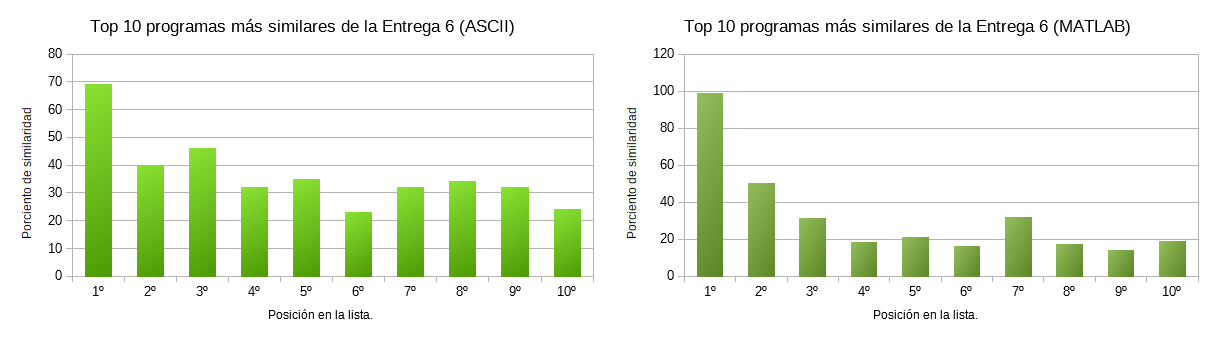
\includegraphics[width=14cm, height=6cm]{imagenes/TOP10_6.png}  %el parámetro scale permite agrandar o achicar la imagen. En el nombre de archivo puede especificar directorios
\caption{10 primeros pares de programas con mayor cantidad de código en común de la entrega 6} \label{fig:TOP10_6}
\end{figure}

\begin{figure}[H] %con el [H] le obligamos a situar aquí la figura
\centering
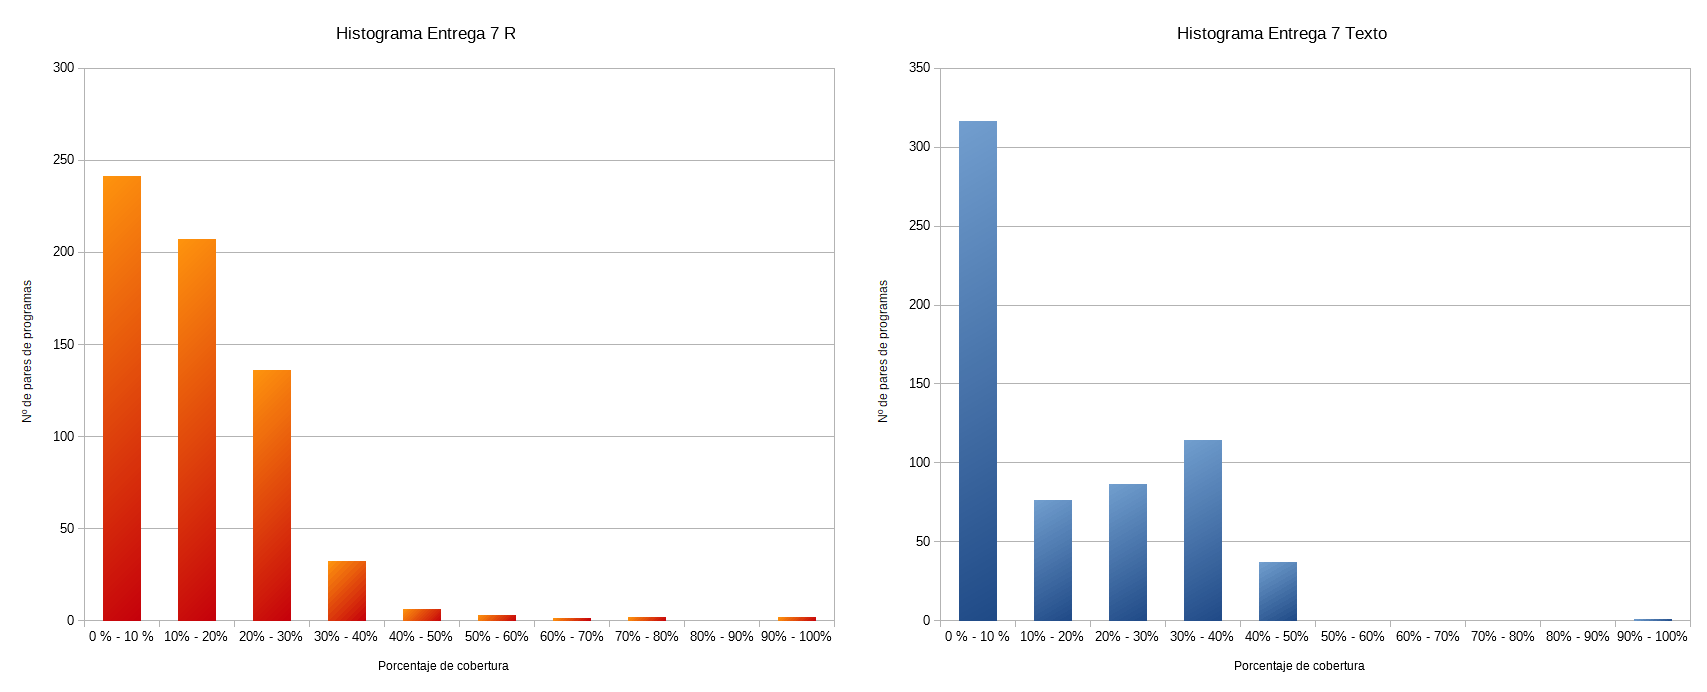
\includegraphics[width=15cm, height=7cm]{imagenes/histograma7.png}  %el parámetro scale permite agrandar o achicar la imagen. En el nombre de archivo puede especificar directorios
\caption{Histogramas de valores de similaridad entre todos los pares de programas de la séptima entrega.} \label{fig:histograma7}
\end{figure}




\begin{figure}[H] %con el [H] le obligamos a situar aquí la figura
\centering
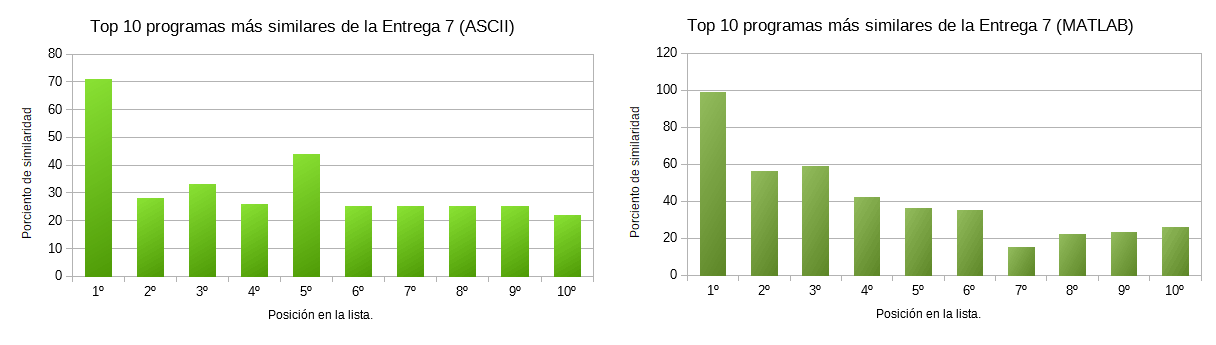
\includegraphics[width=14cm, height=6cm]{imagenes/TOP10_7.png}  %el parámetro scale permite agrandar o achicar la imagen. En el nombre de archivo puede especificar directorios
\caption{10 primeros pares de programas con mayor cantidad de código en común de la entrega 7} \label{fig:TOP10_7}
\end{figure}


Los índices de similaridad son aún más bajos, los altos se deben a comentarios iguales como en los casos anteriores y nuestro frontend sigue detectando los contados plagios debidos a estructuras de control casí iguales.
\newline
\bigskip

Hemos podido comprobar en los resultados obtenidos en las siete entregas que el frontend que hemos creado para JPLAG permite detectar:
\begin{enumerate}
\item Plagios en los que el código se ha copiado entero.
\item Plagios en los que sólo se ha cogido parte del código.
\item Plagios en los que se ha modificado parcialmente el código para ocultar la copia, ya sea cambiando el nombre de variables o usando estructuras de control equivalentes.
\end{enumerate}
Pueden ocurrir falsos positivos con índice de similaridad alto, es por esto que los casos intermedios (entre 30\% y 60\% de similaridad) deben investigarse en mayor profundidad para comprobar si verdaderamente hay ocurrido plagio.
\newline
Para ello tan sólo tendremos que ir a las páginas de comparación de código donde se muestran los fragmentos donde se han detectado estructuras similares o iguales.
\newline
Los casos en los que ha ocurrido plagio y JPLAG con nuestro frontend no lo detecta requieren que el alumno haya modificado hasta tal punto la estructura del archivo que ya no se consideraría plagio, ya que esto significaría que el alumno entiende como funciona perfectamente el código que esta plagiando y sabe por tanto resolver el ejercicio.















